%\newcommand{\thirdFigWidth}{0.15\textwidth}

\begin{figure}[ht!]
%
% \begin{center}
% \centering
\begin{subfigure}[t]{\thirdFigWidth}
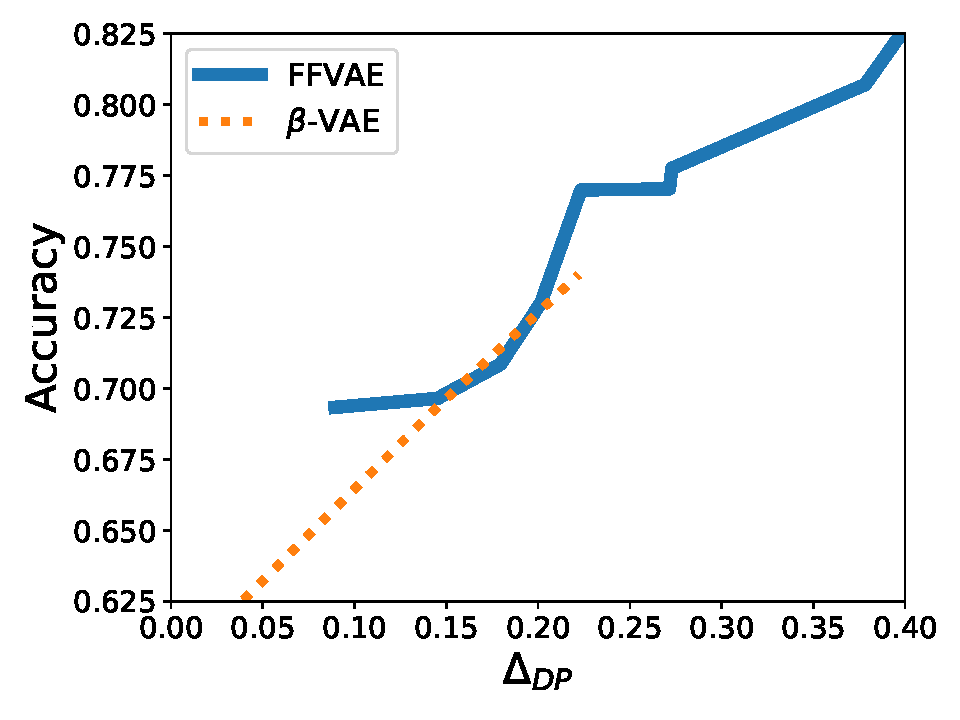
\includegraphics[width=\textwidth]{predict_C.pdf}
\caption{$a$ = C}
\label{fig:predict_C}
\end{subfigure}
%
\hfill
%
\begin{subfigure}[t]{\thirdFigWidth}
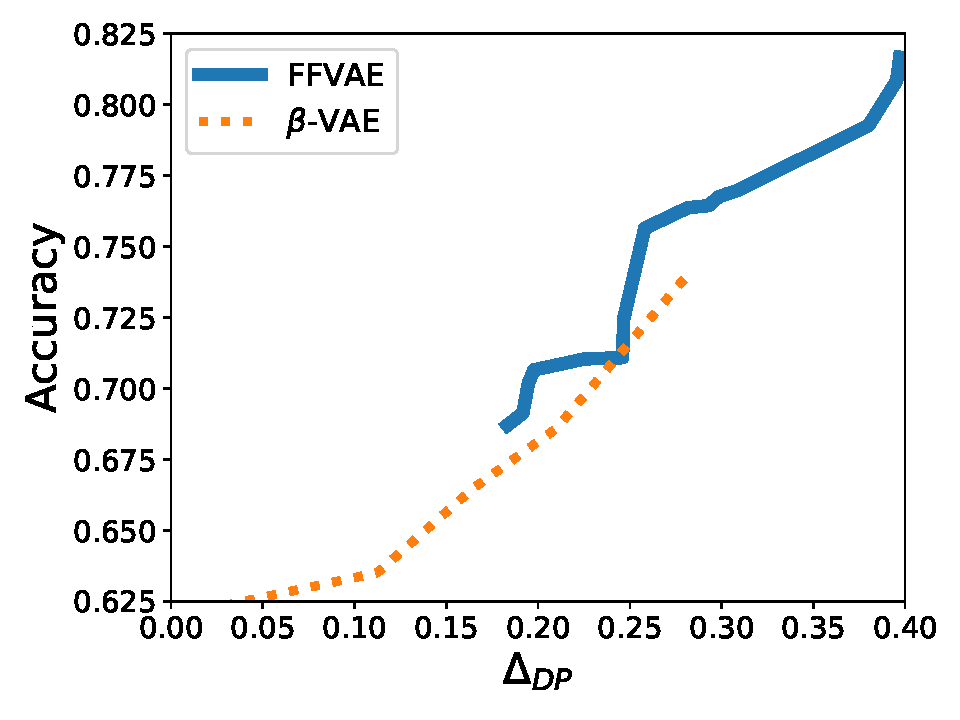
\includegraphics[width=\textwidth]{predict_E.pdf}
\caption{$a$ = E}
\label{fig:predict_E}
\end{subfigure}
%
\hfill
%
\begin{subfigure}[t]{\thirdFigWidth}
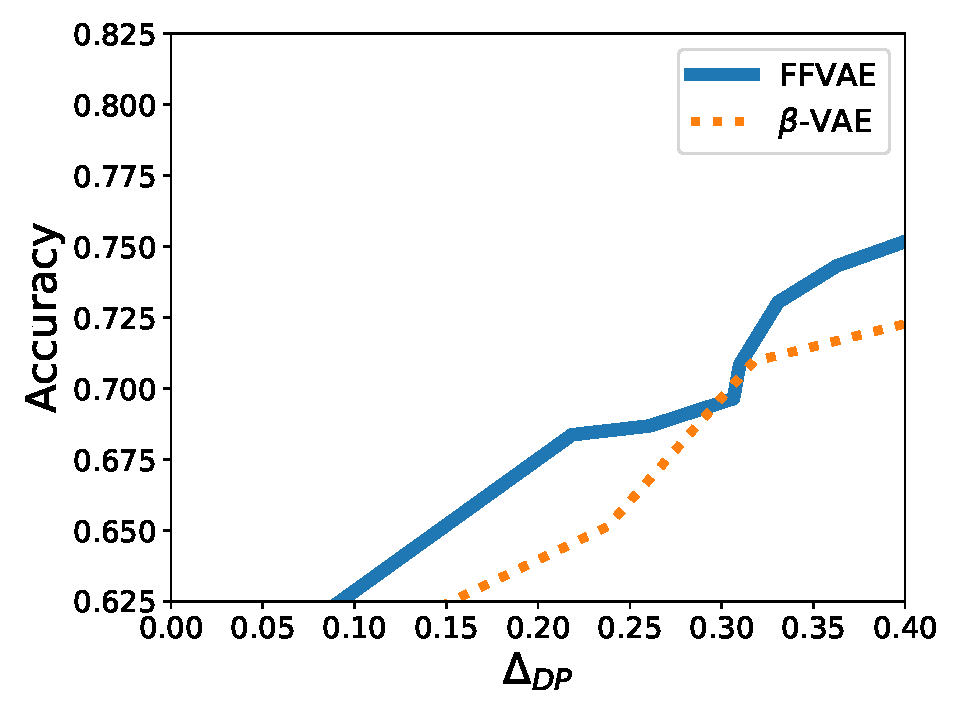
\includegraphics[width=\textwidth]{predict_M.pdf}
\caption{$a$ = M}
\label{fig:predict_M}
\end{subfigure}
%
\hfill
%
\begin{subfigure}[t]{\thirdFigWidth}
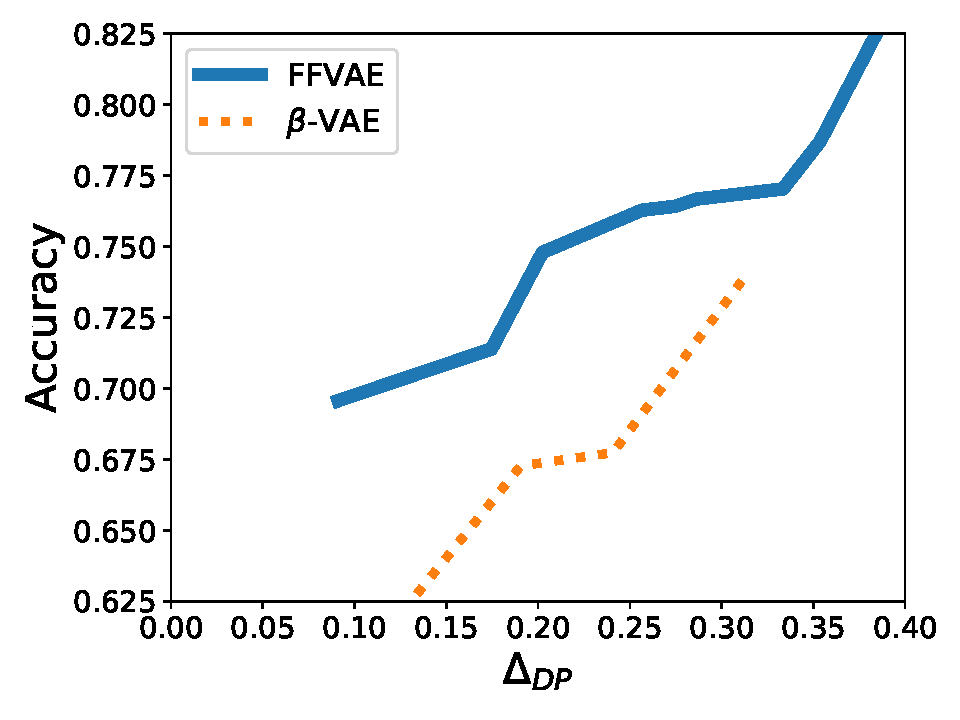
\includegraphics[width=\textwidth]{predict_C-AND-E.pdf}
\caption{$a$ = C $\wedge$ E}
\label{fig:predict_C-AND-E}
\end{subfigure}
%
\hfill
%
\begin{subfigure}[t]{\thirdFigWidth}
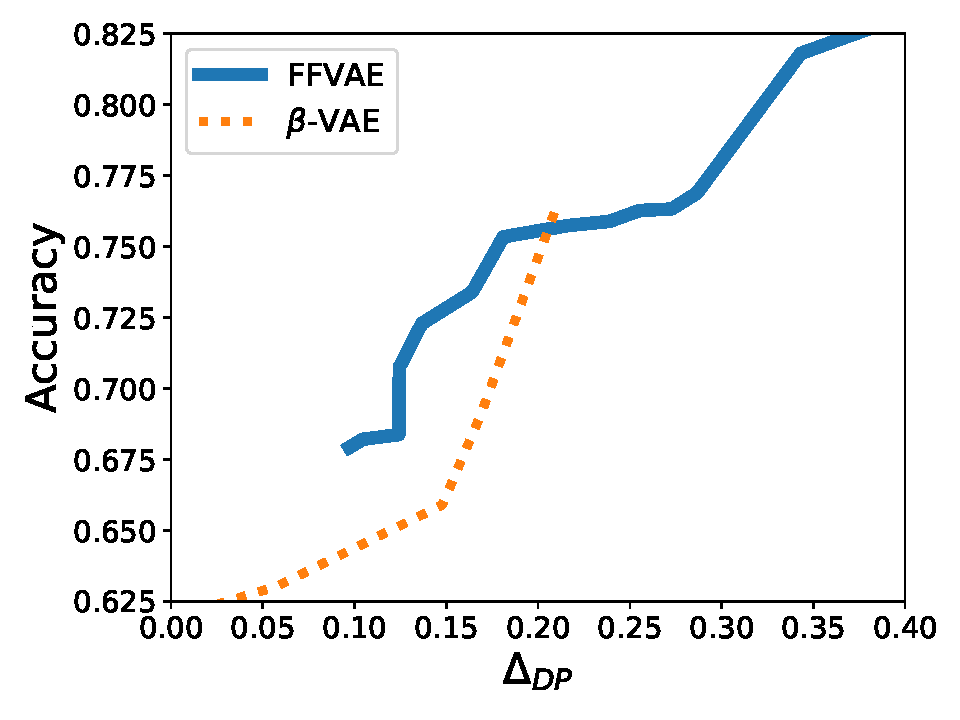
\includegraphics[width=\textwidth]{predict_C-AND-NOT-E.pdf}
\caption{$a$ = C $\wedge \neg$ E}
\label{fig:predict_C-AND-NOT-E}
\end{subfigure}
%
\hfill
%
\begin{subfigure}[t]{\thirdFigWidth}
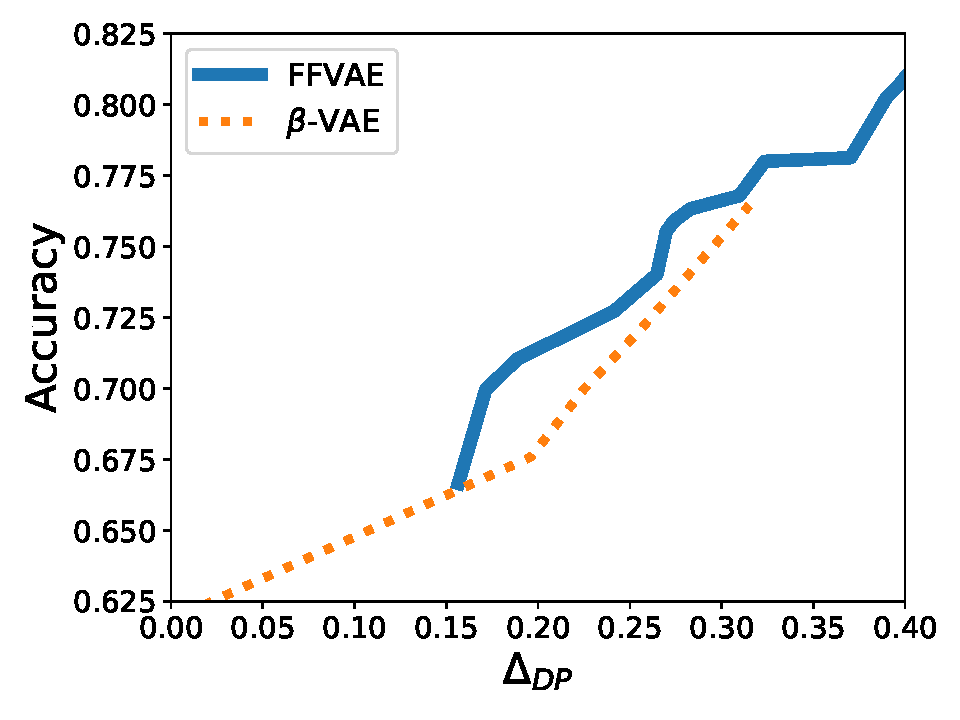
\includegraphics[width=\textwidth]{predict_NOT-C-AND-E.pdf}
\caption{$a$ = $\neg$ C $\wedge$ E}
\label{fig:predict_NOT-C-AND-E}
\end{subfigure}
%
\hfill
%
\begin{subfigure}[t]{\thirdFigWidth}
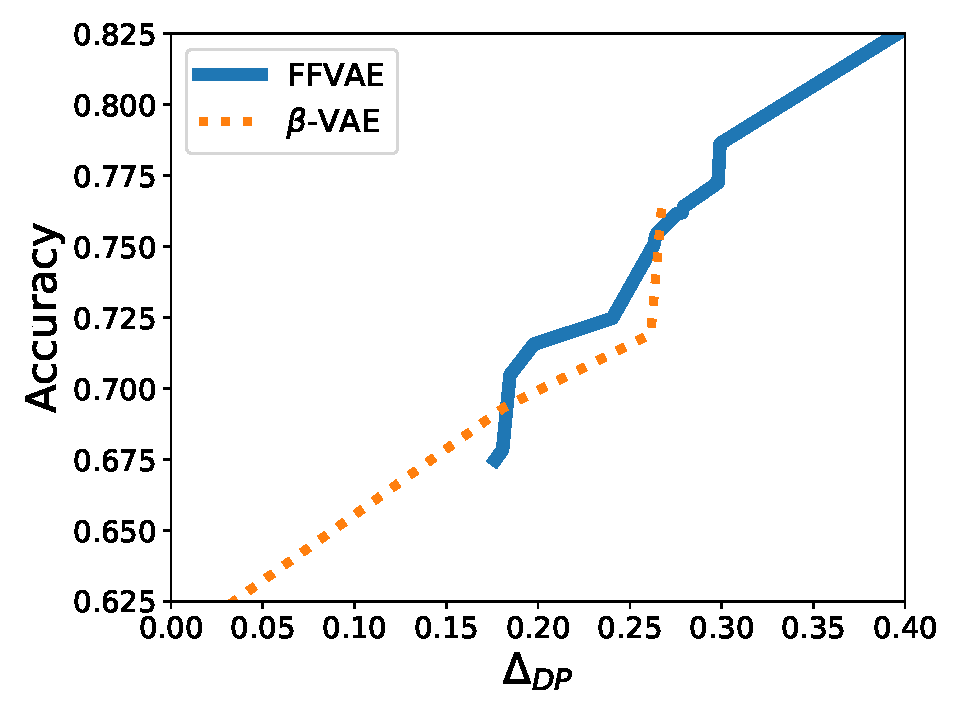
\includegraphics[width=\textwidth]{predict_NOT-C-AND-NOT-E.pdf}
\caption{$a$ = $\neg$ C $\wedge \neg$ E}
\label{fig:predict_NOT-C-AND-NOT-E}
\end{subfigure}
%
\hfill
%
\begin{subfigure}[t]{\thirdFigWidth}
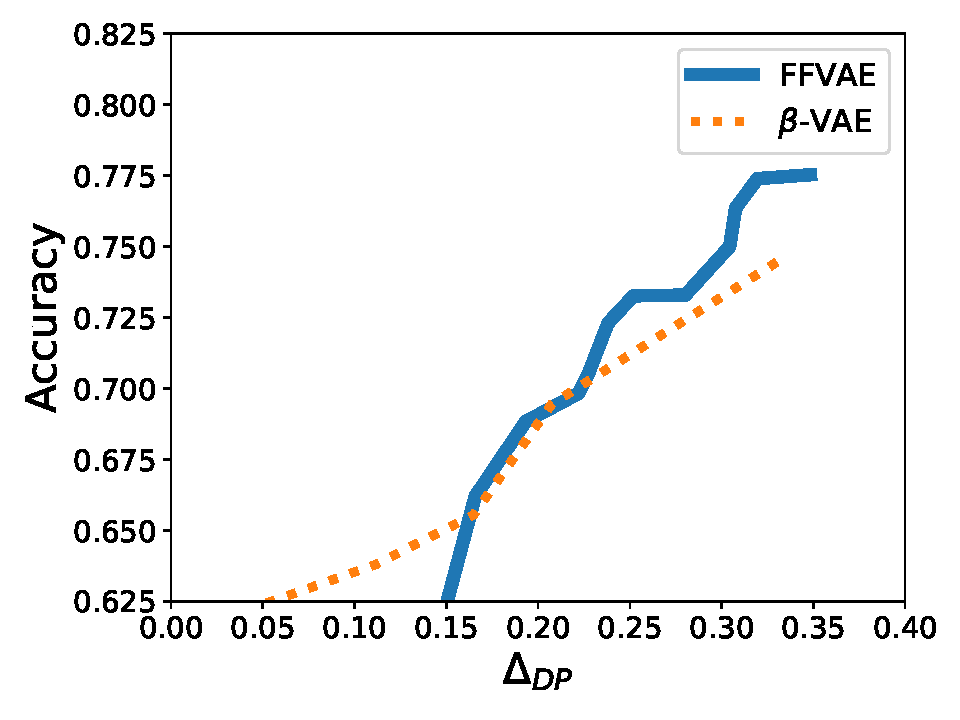
\includegraphics[width=\textwidth]{predict_C-AND-M.pdf}
\caption{$a$ = C $\wedge$ M}
\label{fig:predict_C-AND-M}
\end{subfigure}
%
\hfill
%
\begin{subfigure}[t]{\thirdFigWidth}
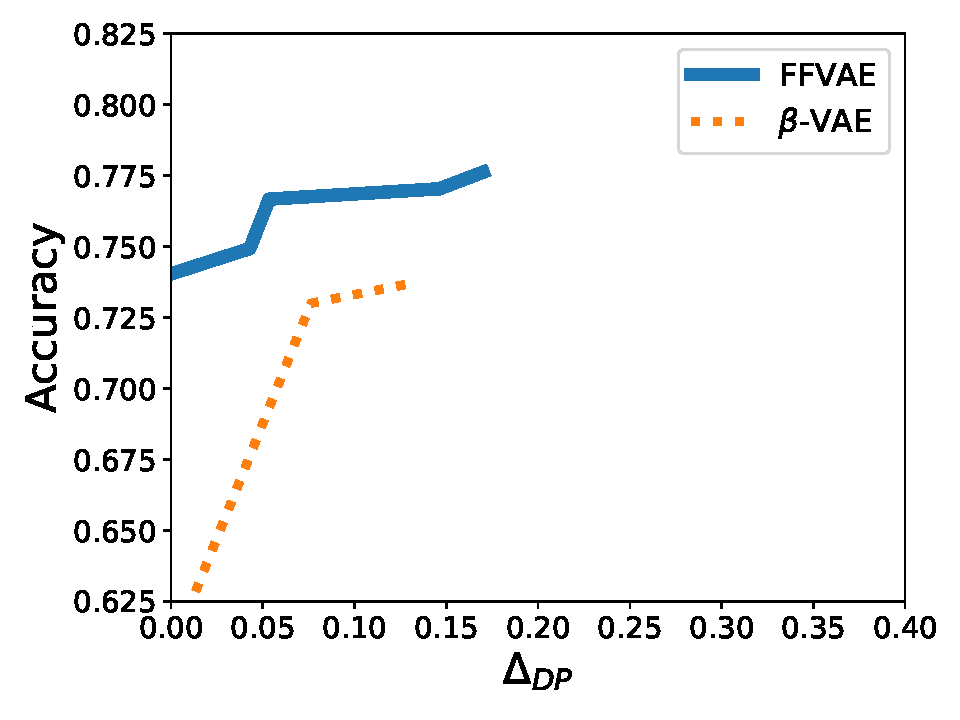
\includegraphics[width=\textwidth]{predict_C-AND-NOT-M.pdf}
\caption{$a$ = C $\wedge \neg$ M}
\label{fig:predict_C-AND-NOT-M}
\end{subfigure}
%
\hfill
%
\begin{subfigure}[t]{\thirdFigWidth}
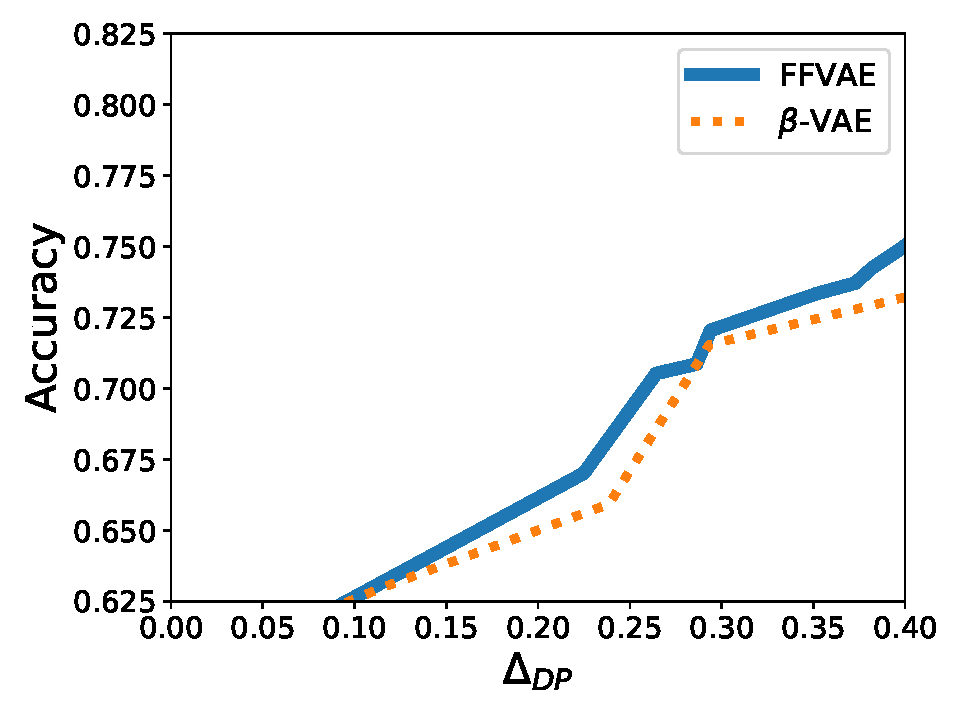
\includegraphics[width=\textwidth]{predict_NOT-C-AND-M.pdf}
\caption{$a$ = $\neg$ C $\wedge$ M}
\label{fig:predict_NOT-C-AND-M}
\end{subfigure}
%
\hfill
%
\begin{subfigure}[t]{\thirdFigWidth}
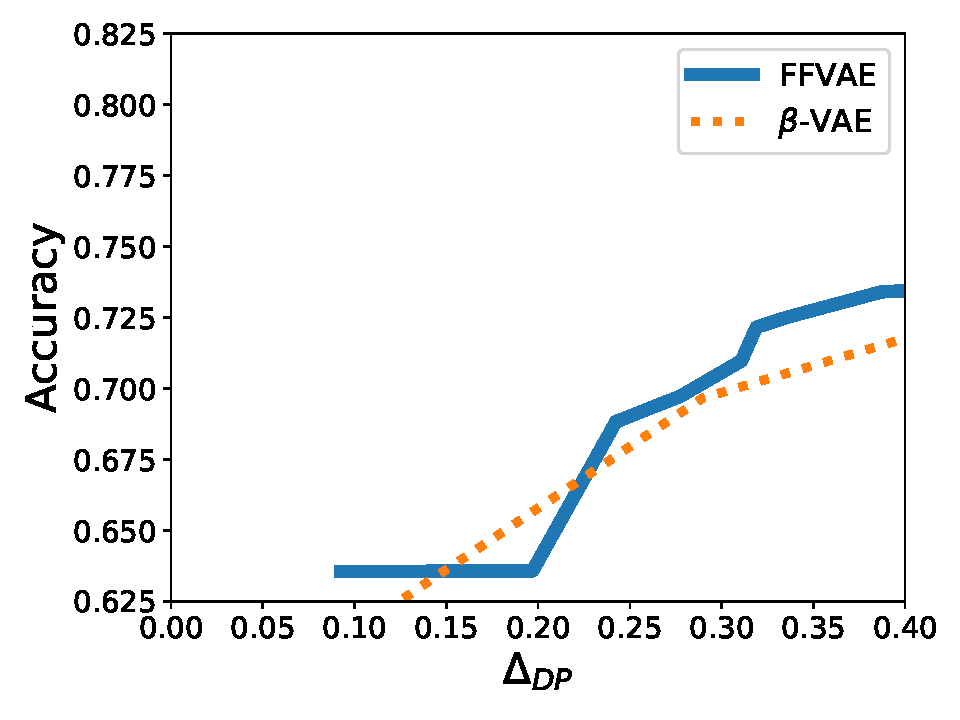
\includegraphics[width=\textwidth]{predict_NOT-C-AND-NOT-M.pdf}
\caption{$a$ = $\neg$ C $\wedge \neg$ M}
\label{fig:predict_NOT-C-AND-NOT-M}
\end{subfigure}
%
\hfill
%
\begin{subfigure}[t]{\thirdFigWidth}
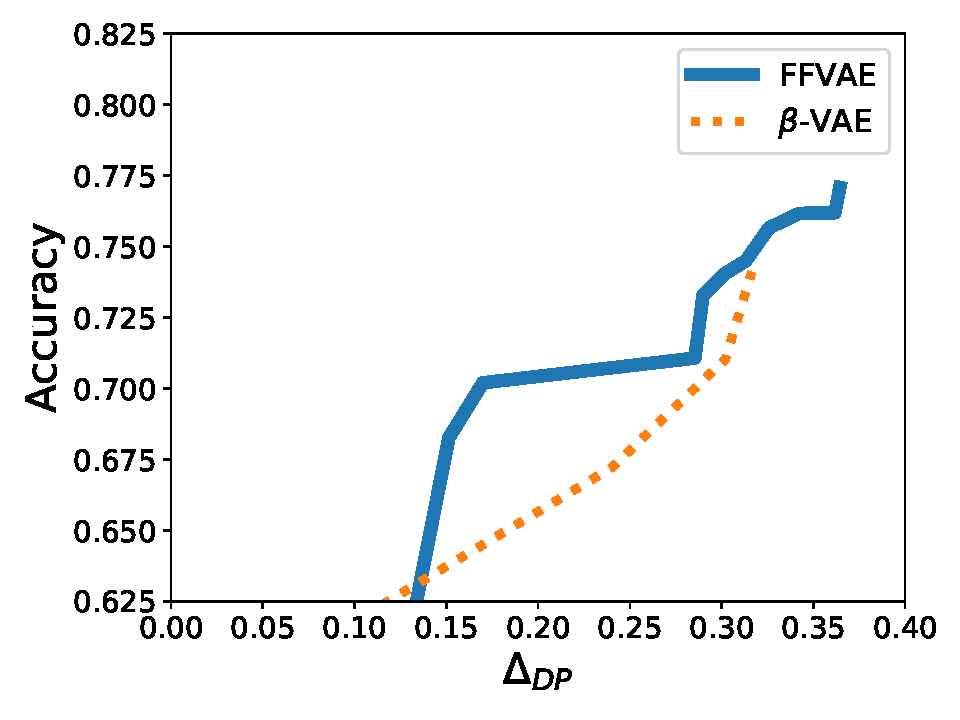
\includegraphics[width=\textwidth]{predict_E-AND-M.pdf}
\caption{$a$ = $\neg$ E $\wedge$ M}
\label{fig:predict_E-AND-M}
\end{subfigure}
%
\hfill

%
\begin{subfigure}[t]{\thirdFigWidth}
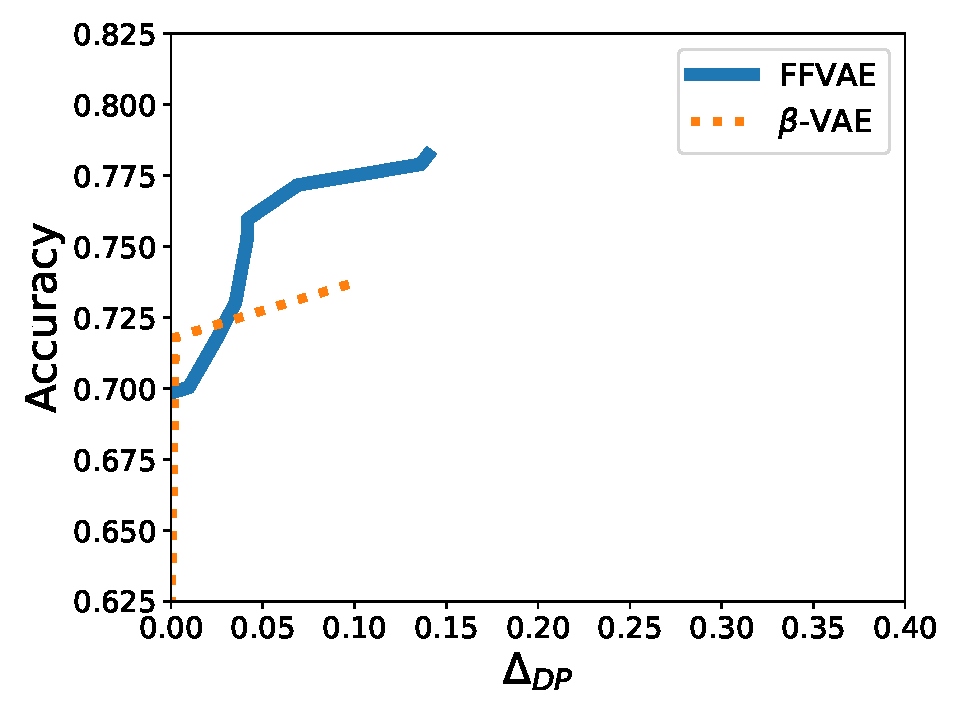
\includegraphics[width=\textwidth]{predict_E-AND-NOT-M.pdf}
\caption{$a$ = E $\wedge \neg$ M}
\label{fig:predict_E-AND-NOT-M}
\end{subfigure}
%
\hfill
%
\begin{subfigure}[t]{\thirdFigWidth}
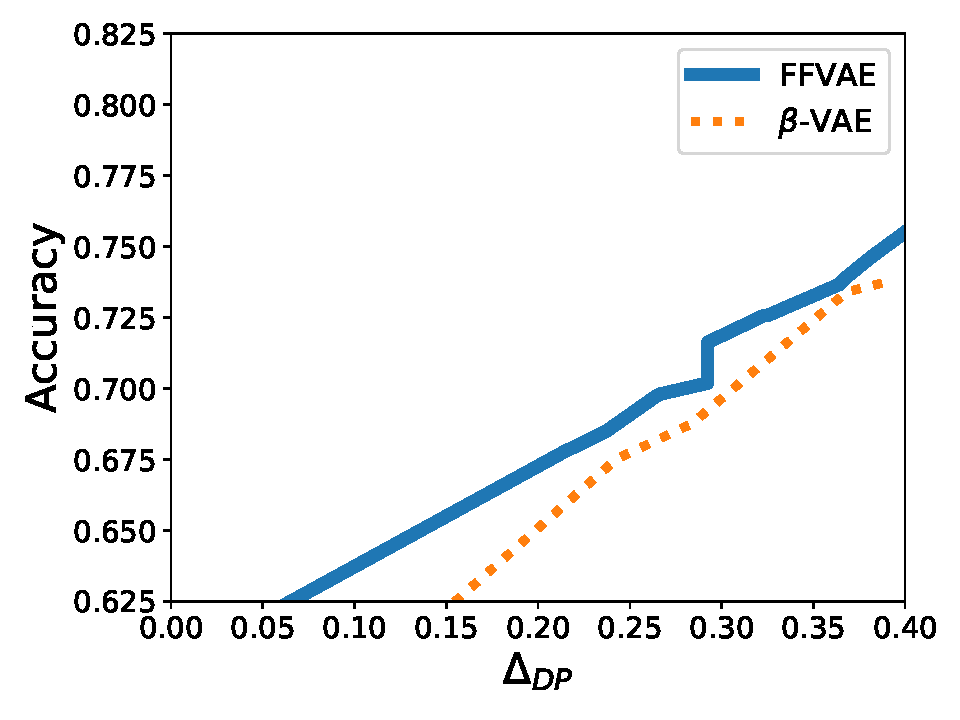
\includegraphics[width=\textwidth]{predict_NOT-E-AND-M.pdf}
\caption{$a$ = $\neg$ E $\wedge$ M}
\label{fig:predict_NOT-E-AND-M}
\end{subfigure}
%
\hfill
%
\begin{subfigure}[t]{\thirdFigWidth}
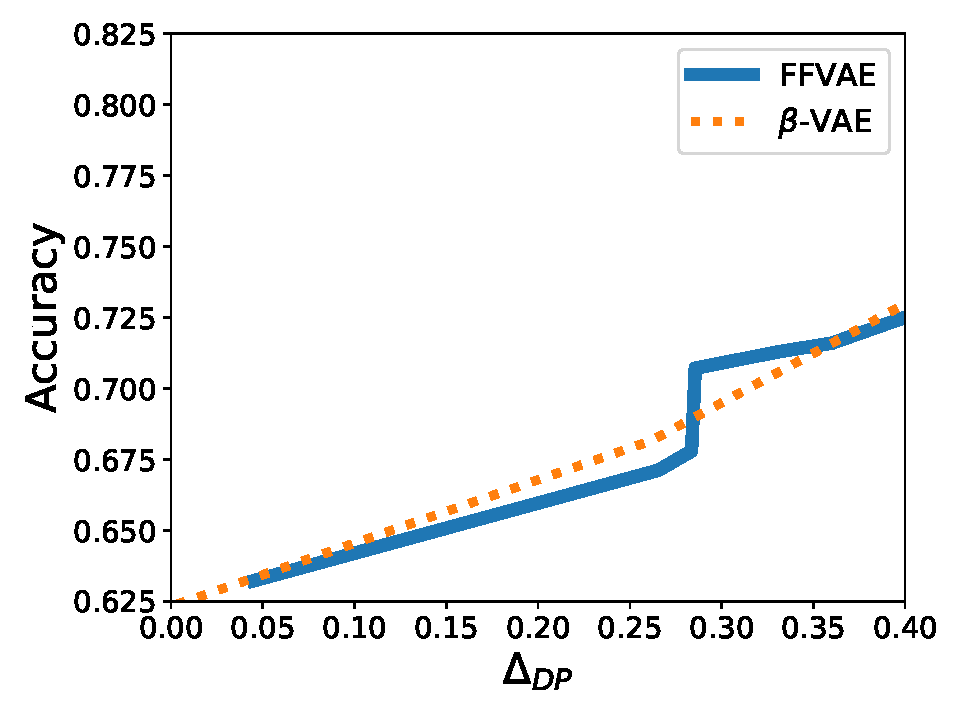
\includegraphics[width=\textwidth]{predict_NOT-E-AND-NOT-M.pdf}
\caption{$a$ = $\neg$ E $\wedge \neg$ M}
\label{fig:predict_NOT-E-AND-NOT-M}
\end{subfigure}
%
\hfill

\caption{
    Celeb-A subgroup fair classification results.
    Sensitive attributes: Chubby (C), Eyeglasses (E), and Male (M).
    $y$ = HeavyMakeup. 
    }
    \label{fig:celeba-pareto}
% \end{center}
% \vskip -0.2in
\end{figure}
